% !TeX root = ../main.tex
\section{Evaluating Textual Choreography}
\label{sec:evaluation}
% !TeX root = ../main.tex
\begin{figure*}[t]
\centering
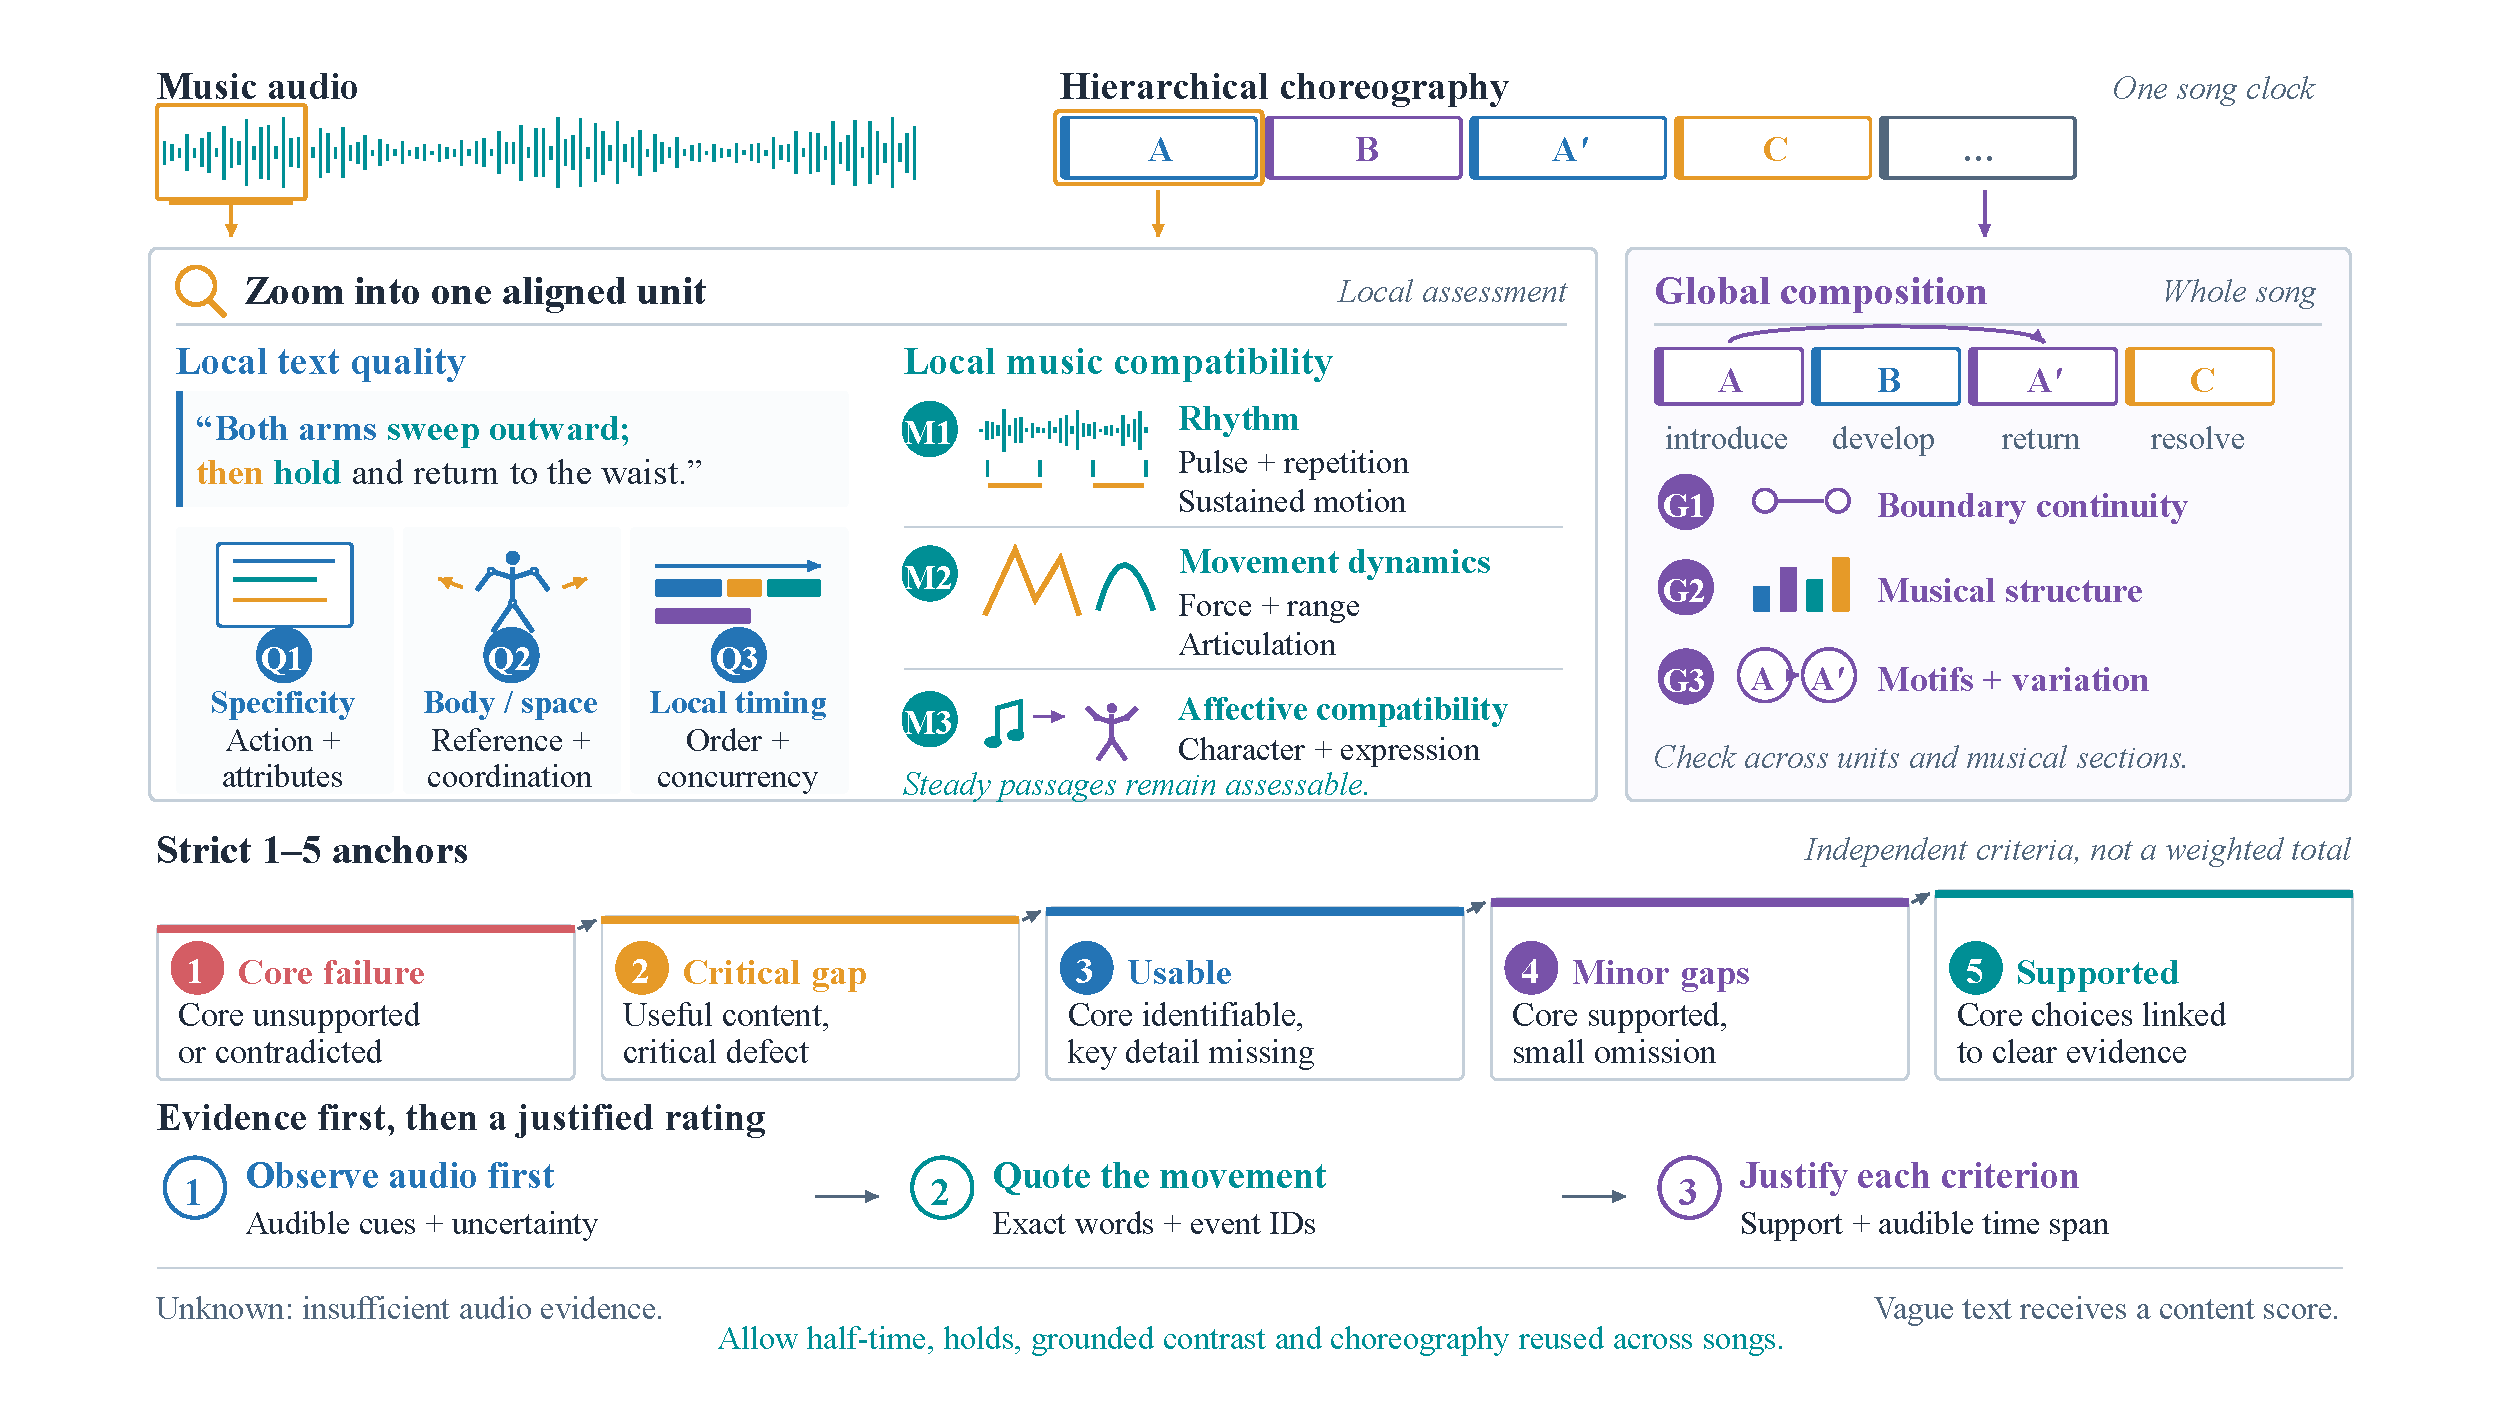
\includegraphics[width=\textwidth]{figures/revision_20261117_v3/paper/evaluation_framework.pdf}
\caption{\textbf{Evidence-grounded evaluation of music and choreography text.}
A single aligned unit supports Q1--Q3 local text quality and M1--M3 music compatibility;
G1--G3 inspect composition across the whole song. The 1--5 anchors require quoted movement
evidence; music-linked claims also require audible support.
M3 assesses affective compatibility, including steady passages.
Unknown denotes insufficient audio evidence, not vague movement text.
Table~\ref{tab:rubric-detailed-anchors} gives the complete guide;
calibration remains pending.}
\label{fig:evaluation-rubric}
\end{figure*}

% Declare the wide results float early so it stays with the main-paper
% experiment discussion rather than being deferred past the conclusion.
% !TeX root = ../main.tex
% Frozen full-2000 aggregates, with BERTScore on the common valid set.
% Requires \usepackage{booktabs}. No model inference was performed.
\begin{table*}[t]
\centering
\caption{Reference agreement on the frozen 2,000-clip choreography panel. BLEU-4 uses a 0--100 scale; other scores are multiplied by 100. BERTScore$^{\dagger}$ uses the common 1,861 valid clips. Higher agreement does not independently establish music alignment or motion quality.}
\label{tab:e2-full2000-v2}
\begingroup
\small
\setlength{\tabcolsep}{3pt}
\renewcommand{\arraystretch}{1.15}
\begin{tabular*}{\textwidth}{@{\extracolsep{\fill}}lrrrrrr@{}}
\toprule
& \multicolumn{4}{c}{Reference text agreement} & \multicolumn{2}{c}{Lexicon agreement}\\
\cmidrule(lr){2-5}\cmidrule(lr){6-7}
Method & BLEU-4 & ROUGE-L & BERT-F1$^{\dagger}$ & Token-F1 & KW-F1 & BP-F1 \\
\midrule
Qwen3-Omni-Instruct & 0.36 & 11.19 & 78.50 & 15.13 & 28.97 & 60.18 \\
MOSS-Audio & 0.73 & 12.77 & 82.64 & 16.32 & 8.76 & 21.31 \\
MOSS-Music & 0.56 & 14.99 & 82.14 & 20.18 & 11.99 & 51.69 \\
Music-Flamingo & 0.85 & 12.79 & 82.29 & 16.11 & 19.67 & 19.46 \\
Audio-Flamingo3 & 0.18 & 7.93 & 82.21 & 9.08 & 9.25 & 12.08 \\
Qwen2.5-Omni & 0.17 & 8.09 & 82.85 & 9.80 & 4.18 & 32.09 \\
\midrule
\textbf{Task-specific SFT (ours)} & \textbf{9.74} & \textbf{30.80} & \textbf{89.71} & \textbf{58.06} & \textbf{80.78} & \textbf{94.12} \\
\bottomrule
\end{tabular*}
\par\vspace{4pt}
\begin{minipage}{\textwidth}\footnotesize
KW/BP: micro-averaged category-set F1 over 39 motion and six body-part
categories. Token-F1: token-multiset overlap. $^{\dagger}$RoBERTa-large,
layer 17, without IDF or baseline rescaling. All remaining metrics use
2,000 clips. Diagnostics and available-case BERTScore appear in
Table~\ref{tab:e2-full2000-diagnostics}. Bold identifies our model.
\end{minipage}
\endgroup
\end{table*}

% Generated by results/build_d123_refinement_table.py from public per-case scores.
\begin{table*}[t]
\centering
\caption{Automatic ratings of our captioning pipeline on a 1--5 scale. r4 and v2.1 are scoring versions applied to the same outputs; v2.1 was defined after earlier tests. Source rating IDs are retained. D4--D6 remain unreported (``--''). Coverage, inference settings, and protocol scope appear in Appendix~\ref{sec:experimental-details}.}
\label{tab:refinement-d123}
\begingroup\small
\setlength{\tabcolsep}{5pt}
\renewcommand{\arraystretch}{1.10}
\begin{tabular*}{\textwidth}{@{\extracolsep{\fill}}llrrrrrr@{}}
\toprule
Method & Rating version & D1 & D2 & D3 & D4 & D5 & D6 \\
\midrule
Ours & r4 & 4.97 & 3.33 & 4.80 & -- & -- & -- \\
Ours & v2.1 & 4.92 & 4.50 & 4.91 & -- & -- & -- \\
\bottomrule
\end{tabular*}
\endgroup
\end{table*}

% Generated by results/build_style_prior_822.py; only the 822-clip population.
\begin{table*}[t]
\centering
\caption{Audio-based dance-style agreement on 822 clips with video-VLM pseudo-labels. MF1: Macro-F1; BA: balanced accuracy. Values are $\times100$; bold marks the highest score per column.}
\label{tab:style-prior-822}
\begingroup\small
\setlength{\tabcolsep}{5pt}
\renewcommand{\arraystretch}{1.08}
\begin{tabular*}{0.90\textwidth}{@{\extracolsep{\fill}}lrrrr@{}}
\toprule
Method & Top-1 & Top-3 & MF1 & BA \\
\midrule
\multicolumn{5}{l}{\emph{Zero-shot audio-language models}} \\
Qwen3-Omni-Instruct & 21.65 & 40.39 & 10.66 & 13.69 \\
MOSS-Audio & 21.17 & 42.70 & 10.41 & 13.79 \\
MOSS-Music & 14.23 & 30.66 & 9.05 & 9.81 \\
Music-Flamingo & 14.23 & 36.01 & 5.07 & 9.00 \\
Audio-Flamingo3 & 12.90 & 38.08 & 2.45 & 8.15 \\
Audio-Flamingo-Next & 15.94 & 25.67 & 5.53 & 10.08 \\
Qwen2.5-Omni & 22.38 & 54.50 & 11.21 & 14.15 \\
\midrule
\multicolumn{5}{l}{\emph{Supervised style heads; frozen MuQ encoder}} \\
MuQ-JEV head: CE & 44.28 & \textbf{81.87} & 29.18 & 29.21 \\
MuQ-JEV head: weighted CE & 41.24 & 77.98 & 29.31 & 30.12 \\
MuQ-JEV head: focal & \textbf{44.77} & 81.39 & \textbf{32.17} & \textbf{32.35} \\
\bottomrule
\end{tabular*}
\endgroup
\end{table*}


\paragraph{Evaluation targets.}
Our music-and-text protocol separates reference agreement, surface
diagnostics, and choreography quality. Connective counts and exact-string
duplication describe surface behavior; neither they nor reference
agreement establish performed synchronization or biomechanics.

\paragraph{Local and whole-song criteria.}
Figure~\ref{fig:evaluation-rubric} groups Q1--Q3 as \emph{local text
quality}, M1--M3 as \emph{local music compatibility}, and G1--G3 as
\emph{global composition}. The figure and
Table~\ref{tab:rubric-detailed-anchors} define integer 1--5 anchors, without
a weighted total: 2 indicates useful content with a critical defect,
3 an important omission, and 4 minor deficiencies. Sustained motion,
half-time, contrast, and intentional recurrence can score highly.
A movement pattern may fit multiple recordings; unique song recovery
is not a quality requirement.
Verbosity and motif labels cannot replace evidence; missing support-foot
information alone is not a contradiction.

\paragraph{Evidence and scoring.}
Ratings require reasons, exact action quotations, and existing event IDs.
M1--M3 and G2--G3 additionally require audible observations with global
timestamps. M3 assesses compatibility between musical character and
bodily expression; it does not require a salient change within a short
window. Ambiguous musical evidence receives \emph{unknown}; a vague
action description instead receives a low score when assessable.
Music observations are obtained before candidates and held fixed across
methods. Service/parsing failures remain separate.

The proposed review contract requires raw responses and checks of types, quotations,
IDs, audio identity, and time bounds. These checks establish format compliance,
not semantic validity, audio coverage, calibration, or listener agreement.

\paragraph{Coverage and aggregation.}
G1--G3 require full-song audio and the complete plan; Q1--Q3 and M1--M3 use crops
with global offsets. A chunk-observation fallback remains unimplemented.

For each method and dimension $d$, $\mathcal V_{sd}$ indexes valid,
assessable regions of song $s$, and $\mathcal S_d$ contains songs with
at least one such region:
\begin{equation}
\label{eq:rubric-aggregation}
\begin{aligned}
\bar r_{sd}&=\frac{1}{|\mathcal V_{sd}|}
                  \sum_{w\in\mathcal V_{sd}}r_{swd},\\
R_d&=\frac{1}{|\mathcal S_d|}\sum_{s\in\mathcal S_d}\bar r_{sd}.
\end{aligned}
\end{equation}
Whole-song dimensions contribute one rating per song. Coverage divides
valid ratings by registered cases, reporting unknown and failed cases
separately. Paired effects use shared valid
regions/songs and song-bootstrap intervals. Completion includes all
registered songs; empty denominators remain undefined.

\paragraph{Controlled validation.}
The prospective controlled protocol fixes beginning/middle/end regions,
evidence, and budgets across Workflow, Self-Refine, ReAct, and our harness.
Calibration and validation require two independent listeners and
cross-family judges. Archived four-criterion, acoustic-summary-only
results (Section~\ref{sec:exp-harness}) assess a different protocol and
cannot validate these audio-conditioned ratings.
